\documentclass[a4paper, 12pt]{article}

% \usepackage[showframe]{geometry}
\usepackage[utf8]{inputenc}
\usepackage{fontspec}
\usepackage{fancyhdr}
\renewcommand\familydefault{\sfdefault}
\usepackage{anyfontsize}
\usepackage{mathtools}
\usepackage[table]{xcolor}
\usepackage{float}
\usepackage{tabularx}
\usepackage{tikz}
\usetikzlibrary{automata, positioning, arrows.meta, shapes}

\tikzset{%
  % >={Latex[width=2mm,length=2mm]},
  % Specifications for style of nodes:
            base/.style = {rectangle, rounded corners, draw=black,
                           minimum width=3cm, minimum height=0.8cm,
                           text centered, font=\sffamily},
            activityStarts/.style = {base, fill=blue!20},
            startstop/.style = {base, fill=red!30},
            manualMode/.style = {base, fill=green!20!red!20},
            autoMode/.style = {base, fill=green!20!red!20},
 }
 \tikzstyle{decision} = [diamond, draw, fill=blue!20!red!20!green!10]
 \tikzstyle{line} = [draw, -stealth, thick]
 

\pagestyle{fancy}
\fancyhf{}
\rhead{}
\lhead{Microprocesadores}
\fancyfoot[RO]{Pag. \thepage}

\renewcommand{\footrulewidth}{0.5pt}

\setcounter{secnumdepth}{0}

\newcommand{\sangria}{\hspace*{1em}}
\newcommand{\Estado}[1]{
  \item[] {\Large {#1}\\ \rule{8em}{0.5pt} }
}
\renewcommand{\contentsname}{Índice}

\begin{document}

\begin{titlepage}

  % \tikz[remember picture, overlay] \node[opacity=0.3,inner sep=0pt] at (current page.center){\includegraphics[width=\paperwidth,height=\paperheight]{background11}};

  \vspace*{5cm}
  \hspace*{0cm}\hfill{\fontsize{35}{40}\selectfont Proyecto de Laboratorio}\\

  \hspace{3cm}\hfill {\fontsize{18}{10}\selectfont Microprocesadores}\\

  \vspace*{2cm}
  \hspace*{3cm}\hfill David Ruiz Barajas 100363683\\
  \hspace*{3cm}\hfill Sergio Vinagrero Gutiérrez 100363693\\

  \hfill Grupo 21
  
  \vspace*{3cm}
  \hfill\includegraphics[width=.6\textwidth]{/home/vinagrero/Templates/UC3M/template/logo_completo_horizontal.png}

\thispagestyle{empty}
\end{titlepage}

\newpage

\tableofcontents
\thispagestyle{empty}

\newpage

\section{Introducción}

En esta memoria se documentará el proceso de diseño y de realización de la práctica de laboratorio de la asignatura de Microprocesadores.\\

Primero se mostrará un esquema de los periféricos utilizados, una explicación de su configuración y uso y por último  un diagrama de flujo que representa los distintos pasos de funcionamiento del proceso para realizar las medidas.

\section{Recursos utilizados}

Para poder llevar a cabo el proyecto, se han utilizado los siguientes periféricos. La configuración completa se puede ver en el archivo Sensor.ioc.

\renewcommand{\arraystretch}{1.9}

\begin{center}
  % \rowcolors{3}{white}{lightgray}
  \setlength{\tabcolsep}{30pt}
  \begin{tabularx}{\textwidth}{m{1em} m{5.6em} X}
    \firsthline
    & \multicolumn{2}{c}{Descripción} \\
    \cline{2-3}
    Periférico & Modo & Uso \\
    \hline
  
    ADC & Continuo & Lectura del valor del potenciómetro\\
    TIM2 & PWM & Movimiento del servo\\
    TIM3 & Input Capture & Lectura de la señal del sensor\\
    TIM9 & Output Compare & Movimiento automático del servo\\
    BUTTON & EXTI & Toma de medidas en el modo manual\\
    USART2 & Asíncrono & Comunicación entre el PC y el microprocesador\\
\lasthline
\end{tabularx}
\label{item:recursos}
\end{center}

El ADC se ha configurado en modo continuo para que tome medidas automáticamente en el modo manual. El problema de esta configuración es que bloquea el resto de procesos y no permite que salten más interrupciones. Para solucionar este problema, se ha bajado el nivel de prioridad del ADC de 0 a 2 para que el resto de interrupciones tengan más prioridad y se permita el correcto funcionamiento del resto del programa.

Otro problema de esta configuración, el cual se comentará posteriormente, es que la toma continua de datos del potenciómetro produce mucho ruido, lo que hace que el servo vibre incluso si no se mueve el potenciómetro. Esto se conoce como \textit{jitter}. Más adelante se propone alguna solución para evitar este problema.\\

Todos los timers utilizados son de 16 bits, lo cual permite una resolución de microsegundos, la cual es suficiente para las funciones para las que se van a utilizar. 

El TIM2 es el utilizado para mover el servo a cualquier posición. Dado que el servo se muevo mediante una PWM donde el ángulo se controla mediante el ciclo de trabajo de la señal. Es por esto que el TIM2 se ha configurado en modo PWM, ya que nos permite posicionar correctamente el servo cambiando el valor del CCR1 de este timer.\\

Para enviar el pulso al sensor de ultrasonidos se ha decidido no usar ningún periférico, excepto un GPIO, ya que el pulso debe durar al menos $10 \mu s$, y esto se puede conseguir fácilmente con una pequeña espera activa. Con esto nos ahorramos el uso de un timer.\\

El TIM3 es el encargado de leer la señal del sensor de ultrasonidos. La señal de este sensor es una señal cuadrada, donde el ciclo de trabajo de dicha onda esta relacionada directamente con la distancia del objeto detectado. La duración máxima de esta señal de este pulso es de 30 ms, pero se ha configurado de manera que el timer cuente hasta 60 ms para evitar problemas.

Se ha configurado el TIM3 como modo de Input Capture con ambos flancos de la señal. Cuando detecta el primer flanco, se guarda el valor del contador en ese instante y se sale de la interrupción. Cuando detecta el segundo flanco, obtenemos de nuevo el valor del contador y por tanto obtenemos la duración de la señal.

De esta manera, solo es necesario utilizar un contador para leer el sensor de ultrasonidos y como la lectura del primer flanco es inmediata, no hay problema de que se pierdan medidas si el objeto esta muy cercano.\\

El botón utilizado es el que viene incorporado en la propia placa, en el pin PA5. Como solo tenemos un botón, no es necesario comprobar que botón ha lanzado la interrupción. Sin embargo, es necesario comprobar que el botón accione la captura de datos solo en el modo manual ya que en el modo automático la captura de datos se acciona mediante el uso de un interruptor.\\

En cuanto a la USART, es el método utilizada para la comunicación entre el PC y el microprocesador. Se utiliza el callback \textit{HAL\_UART\_RxCpltCallback} para saber cuando se ha transmitido información 
\section{Diagrama de funcionamiento}

\begin{figure}[H]
  \centering
   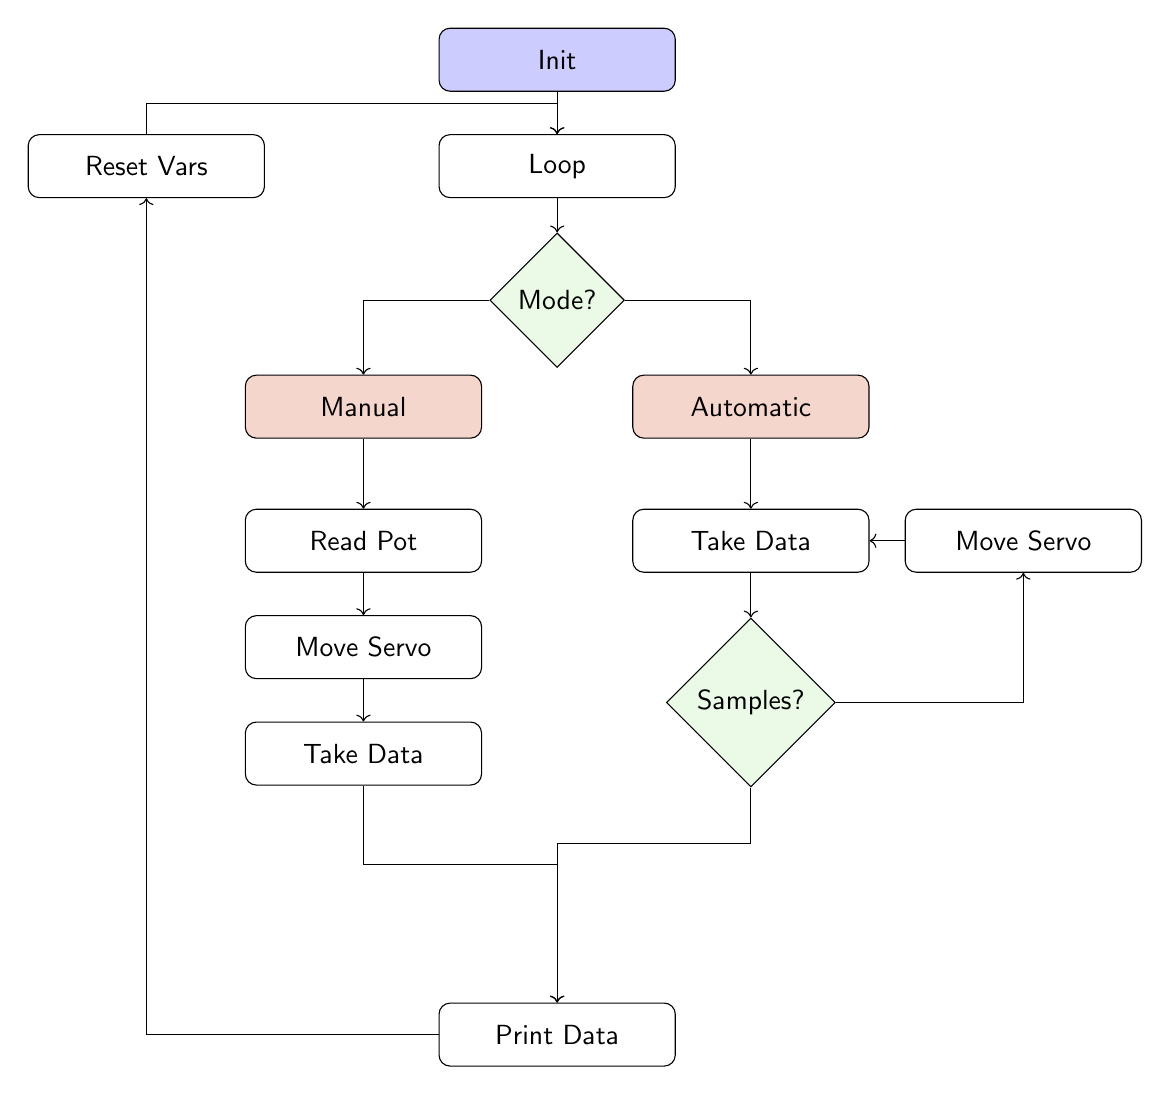
\begin{tikzpicture}[node distance=1cm, every node/.style={fill=white, font=\sffamily}, align=center]
  % Specification of nodes (position, etc.)
     \node (start) [activityStarts] {Init};
     \node (activityRuns) [base, below of=start, yshift=-1em] {Loop};
     \node (modeSel) [decision, below of=activityRuns, yshift=-2em] {Mode?};
     \node (resetVars) [base, left of=activityRuns, xshift=-12em] {Reset Vars};
     
     \node (manualMode) [manualMode, below of=modeSel, xshift=-7em, yshift=-1em] {Manual};
     \node (readPot) [base, below of=manualMode, yshift=-2em] {Read Pot};
     \node (movServoM) [base, below of=readPot, yshift=-1em] {Move Servo};
     \node (takeDataM) [base, below of=movServoM, yshift=-1em] {Take Data};

     \node (autoMode) [autoMode, below of=modeSel, yshift=-1em, xshift=7em] {Automatic};
     \node (takeDataA) [base, below of=autoMode, yshift=-2em] {Take Data};
     \node (numSamples) [decision, below of=takeDataA, yshift=-3em] {Samples?};
     \node (movServoA) [base, right of=takeDataA, xshift=7em] {Move Servo};

     \node (printData) [base, below of=readPot, yshift=-15em, xshift=7em] {Print Data};
     
     
     \draw[->] (start) -- (activityRuns);
     \draw[->] (activityRuns) -- (modeSel);
     
     \draw[->] (modeSel) -| (manualMode);
     \draw[->] (modeSel) -| (autoMode);

     \draw[->] (manualMode.south) -| (readPot.north);
     \draw[->] (readPot.south) -| (movServoM.north);
     \draw[->] (movServoM.south) -| (takeDataM.north);
     \draw[->] (takeDataM.south) --+(0, -1) -| (printData.north);


     \draw[->] (autoMode.south) -| (takeDataA.north);
     \draw[->] (takeDataA.south) -| (numSamples.north);
     \draw[->] (numSamples.east) -| (movServoA.south);
     \draw[->] (movServoA.west) -- (takeDataA.east);
     \draw[->] (numSamples.south) --+(0, -0.71) -| (printData);
     \draw [->] (printData) -| (resetVars);
     \draw [->] (resetVars) --+(0, 0.8) -| (activityRuns.north);

   \end{tikzpicture}
   \label{fig:diagrama}
   \caption{Diagrama de flujo de funcionamiento del programa}
 \end{figure}

 \begin{itemize}

   \newpage
\Estado{Init}
  
  \sangria{} Es el punto de entrada del programa. Se inicia el microprocesador y se configuran los periféricos mediante las librerías de \textit{HAL}.\\
  Seguidamente se llama a la función \textit{user\_init()}, la cual inicia los periféricos a su correspondiente configuración para el funcionamiento en el modo manual. 

\vspace*{2em} 
\Estado{Mode}
  
  \sangria{} Aquí se comprueba el modo de funcionamiento en el que se está trabajando. Para cambiar el modo de funcionamiento se envía el carácter `c' mediante la USART al microprocesador y seguidamente se alterna el modo.\\

  \sangria{} La señal para alternar de modo enviada desde el PC se gestiona desde el callback \textit{HAL\_UART\_RxCpltCallback}. Uno de los problemas de esta implementación es que el sistema no espera a que se haya acabado la medida que se está realizando.\\ Para evitar que se realizan medidas a la mitad, o que el servo no se haya posicionado donde debería, sería conveniente esperar a que el microprocesador haya realizado todas las operaciones y después alternar el modo de funcionamiento.

\vspace*{2em} 
\Estado{Read Pot}
  
  \sangria{} En este estado se lee el ADC para posicionar el potenciómetro de manera manual. El valor del potenciómetro se pasa a fondo de escala para tener el valor real.
  Esta es la interrupción con menos prioridad, ya que de tener la misma prioridad que el resto el programa no saldría de dicha interrupción.\\
  
Una posible mejora en este estado sería un sistema similar al antirebote, mediante el cual solo se permite la toma de datos del ADC cada cierto tiempo, pocos milisegundos por ejemplo, para no saturar el ADC. Esto además también traería la mejora de la reducción del ruido de la lectura del potenciómetro, por lo evitaríamos el \textit{jitter}

\vspace*{2em}
\Estado{Move Servo}

  \sangria{} En este modo tenemos que hacer la distinción entre los modos manual y automático.\\

  En el modo manual, se obtiene la medición del ADC del potenciómetro. Este valor se recorta a los ángulos límites del servo para evitar problemas de sobregiro. Una vez el valor esta en el rango de movimientos validos, el CCR1 del timer con output en PWM encargado de mover el servo se pone a ese valor.
  Como se ha mencionado anteriormente, existe el problema del \textit{jitter}, dado que las pequeñas variaciones del potenciómetro se ven acrecentadas en este estado.\\

  En el modo automático se sigue un hilo de funcionamiento muy similar. Esta vez los valores no se leen del potenciómetro, sino que son modificados mediante el uso de un timer, el cual salta cada 500 ms. El sensor realiza un barrido con 5 muestras. Este numero se puede ver en la variable \textit{NUM\_SAMPLES} en el fichero \textit{main.h}.
  Teniendo el numero de muestras a realizar y los ángulos limite del servo, se calcula de que tamaño es el incremento. Este incremento se refiere al CCR1 del timer encargado de mover el servo.

  
\vspace*{2em}
\Estado{Take Data}

\sangria{} Este estado es el encargado de tomar y guardar las medidas. Para almacenar las medidas se han utilizado dos arrays estáticos tan grandes como el número de medidas a realizar. Un array es para las distancias, y otro es para el ángulo del servo.

En el modo manual, se guardan las medidas en la primera posición y no se permiten más medidas. En el modo automático se hace uso de un contador de muestras, el cual se incrementa cada vez que se hace una medida.
Una vez se ha tomado una mediad en el modo manual o se ha realizado el barrido completo, se habilita la muestra de datos por pantalla.

\newpage
\Estado{Print Data}
  
  \sangria{} Una vez se han capturado todos los datos, estos se muestran por pantalla mediante el puerto serie.
  Se muestra la distancia medida y el ángulo al que se realizo dicha medida.\\
  
  Como el sensor tiene un rango de funcionamiento de entre 2 y 400 centímetros, si una medida se toma fuera de ese rango se indica al usuario que la medida realizada esta fuera de rango.

\vspace*{2em}
\Estado{Reset Vars}

  \sangria{} Es el estado final cuando se ha realizado un ciclo del proceso. Aquí se configuran todas las flags y se resetean las variables de control del proceso. Este estado permite que solo se muestren por pantalla las medidas realizadas una vez se ha completado el ciclo de trabajo.

\end{itemize}


\end{document}



